%
% Complete documentation on the extended LaTeX markup used for Insight
% documentation is available in ``Documenting Insight'', which is part
% of the standard documentation for Insight.  It may be found online
% at:
%
%     http://www.itk.org/

\documentclass{InsightArticle}


%%%%%%%%%%%%%%%%%%%%%%%%%%%%%%%%%%%%%%%%%%%%%%%%%%%%%%%%%%%%%%%%%%
%
%  hyperref should be the last package to be loaded.
%
%%%%%%%%%%%%%%%%%%%%%%%%%%%%%%%%%%%%%%%%%%%%%%%%%%%%%%%%%%%%%%%%%%
\usepackage[dvips,
bookmarks,
bookmarksopen,
backref,
colorlinks,linkcolor={blue},citecolor={blue},urlcolor={blue},
]{hyperref}
% to be able to use options in graphics
\usepackage{graphicx}
% for pseudo code
\usepackage{listings}
% subfigures
\usepackage{subfigure}


%  This is a template for Papers to the Insight Journal. 
%  It is comparable to a technical report format.

% The title should be descriptive enough for people to be able to find
% the relevant document. 
\title{Openings and closing by unions and intersections}

\newcommand{\IJhandlerIDnumber}{0000}

% Increment the release number whenever significant changes are made.
% The author and/or editor can define 'significant' however they like.
\release{0.00}

% At minimum, give your name and an email address.  You can include a
% snail-mail address if you like.
\author{Richard Beare}
\authoraddress{Richard.Beare@monash.edu\\Department of Medicine\\Monash University\\Melbourne\\Australia}

\begin{document}

\IJhandlefooter{\IJhandlerIDnumber}

\maketitle

\ifhtml
\chapter*{Front Matter\label{front}}
\fi


\begin{abstract}
\noindent
Openings by unions of line segments or closings by intersections of
line segments\cite{Serra82} are useful tools that provide a way to filter image
structures based on their length. This article introduces ITK classes
implementing these filters.
\end{abstract}

\tableofcontents

\section{Introduction}
A standard morphological opening by, for example, a square structuring
element removes image structures in which the structuring element will
not fit. This means that a bright regions smaller than the structuring
element will be removed. A closing by the same structuring element
will fill dark regions that are smaller than the structuring element.

If the image contains narrow structures and blobs then it is difficult
to remove one while retaining the other using standard structuring
elements. An alternative is to apply an opening by union (pixel wise
maxima) of multiple line structuring elements oriented at varying
angles. This will remove blobs that cannot contain any of the
structuring elements while retaining lines that can contain at least
one structuring element.

\section{OpenBunImageFilter and CloseBinImageFilter}
The two filters implementing opening by union and closing by
intersection are {\em itk::OpenBunImageFilter} and {\em
  itk::CloseBinImageFilter}. They share a parent class named {\em
  itk::VanHerkGilWermanOpenCloseLineImageFilter} and extend the
infrastructure and utilities provided by the ITK morphology tools. In
particular, they use the {\em itk::FlatStructuringElement} to
represent the lines along which openings and closings will be applied.

Standard usage is:
\lstinputlisting{../openbunTest.cxx}

\section{Examples}
Lets begin with a synthetic example illustrated in Figure
\ref{fig:source_and_open} and available in the CMake tests. The length
of the line is greater than the diameter of the circle so an opening
by union of lines of length between the circle diameter and the
vertical line will remove the circle but retain the line. A single
flat structuring element wider than the line would remove the line, so
one that would remove the circle would also remove the line.
\begin{figure}[htbp]
\centering
\subfigure[Input]{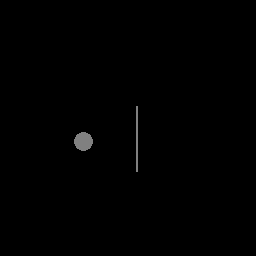
\includegraphics[scale=0.75]{circle_line}}
\subfigure[Output]{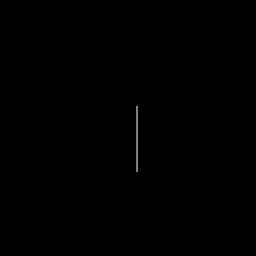
\includegraphics[scale=0.75]{circlineOpen}}
\caption{Synthetic example with circle and line before and after openbun using lines of length 21 pixels.\label{fig:source_and_open}}
\end{figure}

\bibliographystyle{plain}
\bibliography{local,InsightJournal} \nocite{ITKSoftwareGuide}

\end{document}

